\section{Introduction}



%









Inspired by the classical theory of stochastic convex optimization \citep{ruppert1988efficient,polyak1992acceleration}, many Language Model (LM) pipelines use some form of model averaging, such as an exponential moving average (\ema) of training iterates, to stabilize optimization and improve the performance of the returned model \citep{izmailov2018averaging,kaddour2022stop,block2025ema,block2024butterfly,busbridge2023scale,olmo20242,lambert2024tulu,wortsman2022model,smollm2}.  A vast body of work has been devoted to understanding LM training, but the ubiquity of iterate averaging in practice raises a fundamental question: \emph{given that an averaged LM will be returned, how should we change training to improve the performance of this average?}

While prior work has implicitly addressed this question by observing that iterate averaging can allow for more aggressive training through higher learning rates or more limited learning rate decay \citep{defazio2024schedule,block2024butterfly,block2025ema}, in this work, we take a direct approach by asking whether we can design a simple modification to the base optimization algorithm that explicitly controls the training trajectory to improve the performance of the iterate-average estimator.  Our starting point is to follow \citet{block2025ema} and observe that once we commit to returning an average of the training trajectory, the optimization algorithm is no longer just producing a final iterate, but rather a statistic of the entire trajectory: we may thus rephrase our key question by asking how we can best modify the training trajectory so as to make the returned model average maximally close to the optimum.

To answer this question, we take a principled approach to algorithm design by deriving a new optimization algorithm from an optimal-control formulation of a stochastic quadratic optimization problem.  Indeed, while LM training is obviously not quadratic, many recent works have derived practically effective optimization interventions by designing algorithms in analytically tractable settings such as convex, quadratic, or linear problems \citep{vyas2024soap,zhang2019lookahead,gupta2018shampoo,block2025ema,duchi2011adaptive}.  In particular, our derivation begins in a deliberately simplified setting: continuous-time stochastic gradient descent on a quadratic objective with additive noise, where the `modification' is realized as an additive \emph{control}.  
In this model, the uncontrolled dynamics reduce to the familiar Ornstein--Uhlenbeck approximation of noisy gradient descent near a quadratic minimum \citep{mandt2015continuous,block2025ema,kutoyants2004statistical}.  We then add a control input to the dynamics and choose this input to minimize the squared error of the returned iterate average, subject to a quadratic penalty on the size of the intervention.  This gives a linear-quadratic stochastic control problem \citep{georgiou2013separation,yong1999stochastic,kwakernaak1972linear}.  Solving this problem yields an optimal controller with a natural interpretation: the algorithm should pull the live iterate toward an estimate of the optimum and toward consistency with the accumulated average of the trajectory. 




\begin{figure}[t]
    \centering
    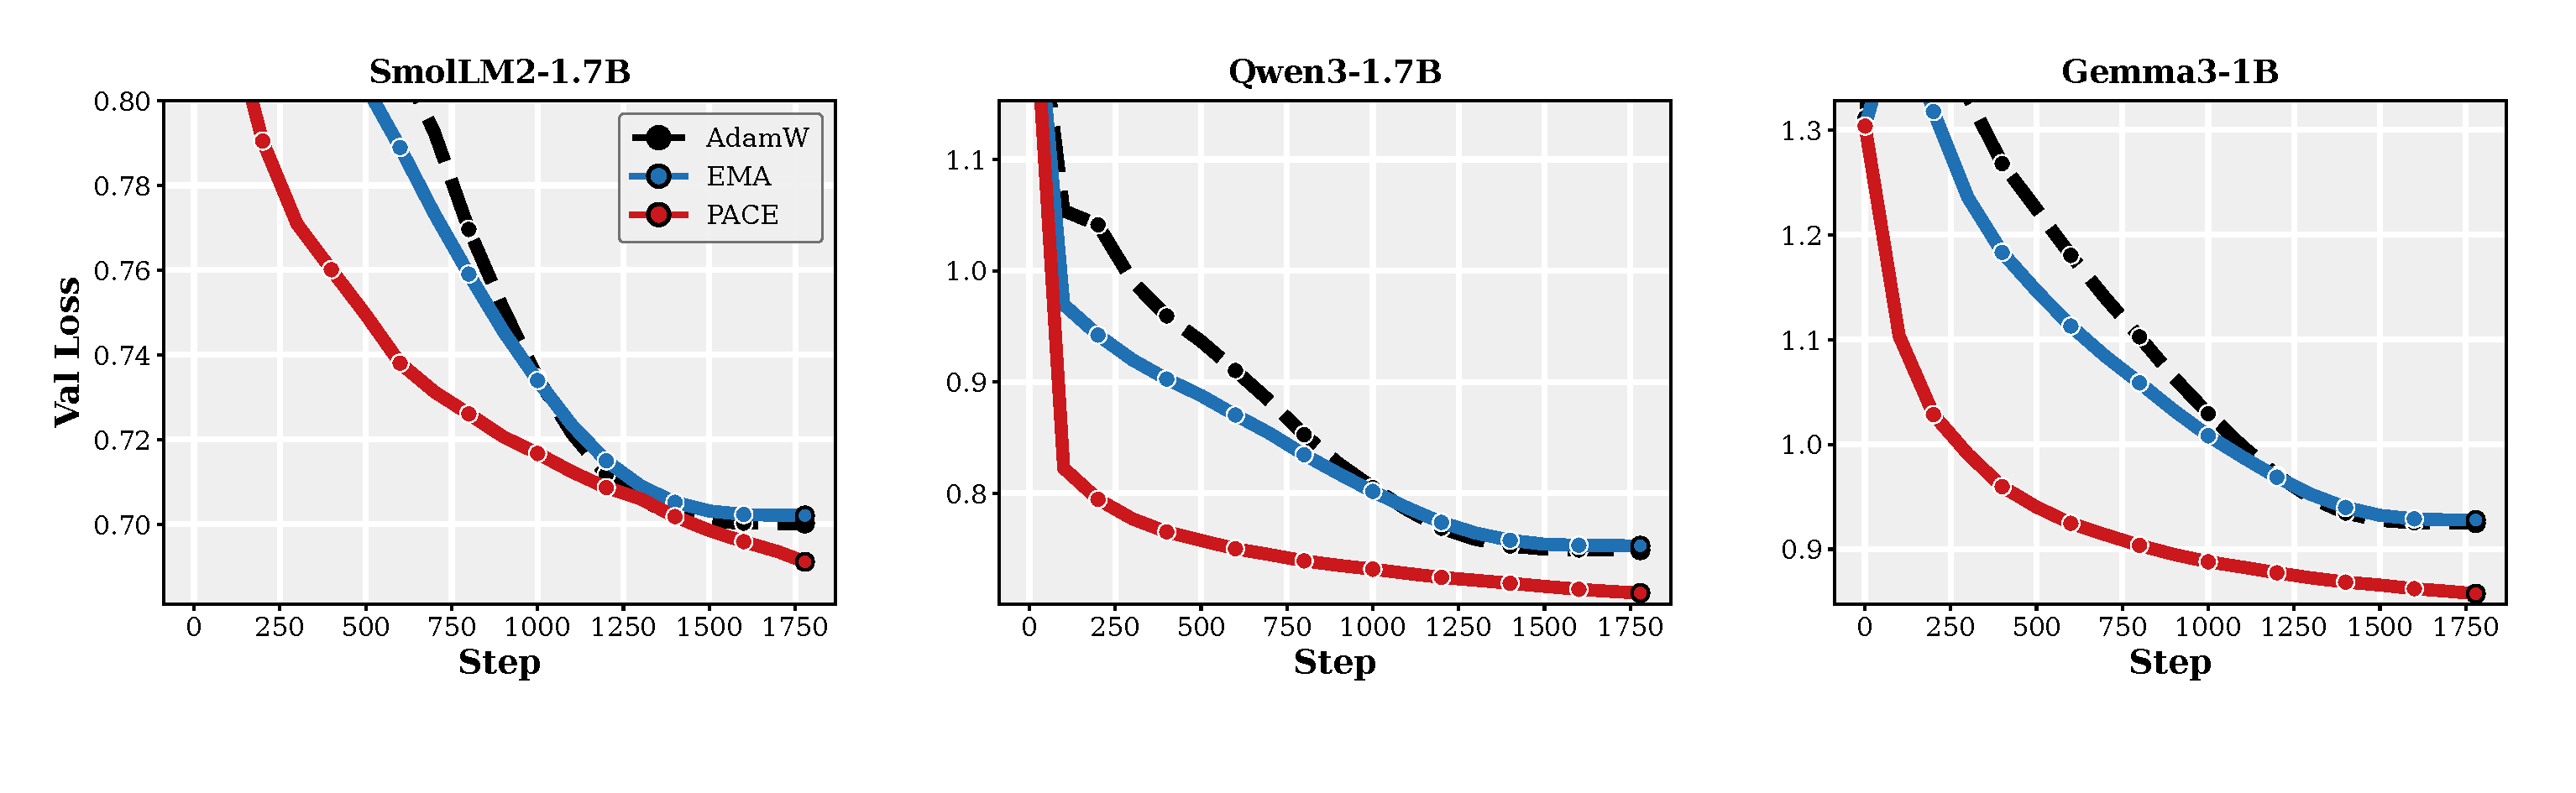
\includegraphics[width=\textwidth]{figures/fig1_best_per_method.pdf}
    \caption{
        \textbf{Performance of \pace\ on fine-tuning.} Validation cross-entropy on \texttt{smol-smoltalk} for SmolLM2-1.7B (\textbf{left}), Qwen3-1.7B (\textbf{middle}), and Gemma3-1B (\textbf{right}).  For each model, \pace\ uses a constant learning rate, while the AdamW and \ema\ baselines use their best learning-rate-decay schedule (cosine or WSD).  \pace\ strictly improves on both baselines on all three models; see \Cref{fig:appendix_multiseed_robust} for a three-seed robustness study.}
    \label{fig:train_curves}
\end{figure}





The exact optimal controller is not directly implementable in modern LM training because it depends on quantities unknown to the learner.  We therefore turn the controller into a practical algorithm through a sequence of heuristic approximations.  We call the resulting method \pace\ (\Cref{alg:controlled-bema}), a lightweight wrapper around AdamW \citep{loshchilov2017fixing} that pays an additional memory cost of model weights in order to better stabilize the training process.  Because \pace\ is derived in such a simplified setting, it is not a priori obvious whether the resulting algorithm has any concrete theoretical guarantees.  We show that a stylized version of the algorithm has convergence guarantees for general convex losses with unbiased stochastic gradients:

\begin{theorem}[Informal version of \cref{thm:convex_convergence}]\label{thm:convex_convergence_informal}
    For any convex loss with unbiased stochastic gradients, the iterate-average estimator returned by \pace\ converges to the minimum at the standard stochastic convex optimization rate, up to a factor depending on the strength of the \ema.
\end{theorem}
In essence, \Cref{thm:convex_convergence_informal} shows that our proposed method is never much worse than SGD for convex objectives, even when the quadratic assumption used in the derivation is dropped.  We then show that, in the quadratic setting from which the algorithm was derived, the controlled dynamics can strictly improve the limiting squared error of the iterate-average estimator relative to the uncontrolled dynamics, and that this improvement can be arbitrarily large on certain quadratic instances:
\begin{proposition}[Informal version of \cref{prop:improved_convergence_quadratic,prop:arbitrarily_large_improvement}]\label{prop:quadratic_improvement_informal}
    In the quadratic setting from which \pace\ is derived, the optimal control strategy can strictly improve the limiting squared error of the iterate-average estimator relative to the uncontrolled dynamics, and this improvement can be arbitrarily large on certain quadratic instances.
\end{proposition}
\iftoggle{colt}{}{
To summarize, in theory, \pace\ is never that much worse than SGD for convex objectives, but can be much better when the objective is locally quadratic.
}

We complement our theory with experiments on LM fine-tuning and pretraining, results of the former of which can be seen in \Cref{fig:train_curves}.  In particular, across three different models of size between 1B and 2B parameters, we find that \pace\ strictly improves over both AdamW and an \ema\ thereof.  In \Cref{sec:experiments}, we present a more detailed analysis of the performance of \pace\ across a range of hyperparameters as well as explore the efficacy of \pace\ on a small pretraining setup at the Chinchilla-optimal token budget \citep{hoffmann2022chinchilla}.  We find that \pace\ is competitive with the Schedule-Free algorithm of \citet{defazio2024schedule}, which also uses iterate averaging to stabilize training and remove the need for learning rate decay and that \pace\ remains competitive with AdamW even when the latter is allowed to decay the learning rate to zero, suggesting that \pace\ can stabilize training in a regime that is not subject to learning rate decay.  \iftoggle{colt}{We now briefly summarize some related works, before moving on to the formal problem setup, algorithm derivation, and rigorous guarantees in \Cref{sec:theory}.}{

\paragraph{Related work.} We now briefly discuss some of the key related works, before moving on to the formal problem setup, algorithm derivation, and rigorous convergence guarantees in \Cref{sec:theory}.
}

\paragraph{Iterate averaging in deep learning.} Originally introduced from the theory of stochastic convex optimization \citep{ruppert1988efficient,polyak1992acceleration}, iterate averaging has been shown to be a powerful tool for stabilizing optimization and improving generalization in deep learning \citep{izmailov2018averaging,kaddour2022stop,block2025ema,block2024butterfly,busbridge2023scale}.  Many approaches have been proposed, including stochastic weight averaging \citep{izmailov2018averaging}, exponential moving averages, and even more complex schemes like model soups \citep{wortsman2022model} and virtually all modern open-source LMs used some form of iterate averaging \citep{smollm2,olmo20242,lambert2024tulu}.  As in our work, there has been much literature on using continuous-time analysis to understand the behavior of iterate averaging in deep learning \citep{busbridge2023scale,mandt2015continuous,malladi2022sdes,block2024butterfly}, with \citet{block2025ema} being the most directly relevant to the present paper.  Unlike that work, which uses continuous-time analysis in a noisy quadratic model to propose a new averaging scheme, here we commit to the standard exponential moving average and instead use continuous-time analysis to design a new optimization algorithm that explicitly controls the training trajectory to improve the performance of this standard averaging scheme.

\paragraph{Comparison to similar optimizers.} Several authors have proposed analyzing optimization through the lens of control theory \citep{lessard2016analysis,davtyan2022koala,xia2025koala}, although the former primarily investigates convergence bounds of existing optimizers and the latter two use the Kalman filter to derive an optimization intervention that, while interesting, does not appear to scale to LMs of modern size.  With regard to the final algorithm, several prior optimizers have similar update rules.  \citet{zhang2015deep,pagliardini2024ademamix} also consider averaging during training (instead of in an offline, post-hoc manner).  The former applies averaging to gradients as opposed to iterates and can be thought of as a more sophisticated version of momentum, whereas the latter has a very different update rule from \pace\ and is intended to solve communication bottlenecks in distributed training.
The authors of \citet{zhang2019lookahead} propose a method that takes gradient steps and periodically transports the live weights toward a slow-moving EMA; our approach recovers a similar update when the pullback value is large, although empirically we find that \pace\ improves performance with intermediate pullback values, improving on that prior work.  Of greatest relevance is the schedule-free (SF) update proposed by \citet{defazio2024schedule}, which also uses iterate averaging to stabilize training and remove the need for learning rate decay, although that work proposes a different algorithm.  Our method is competitive with SF empirically, although pays for improved theoretical convergence in the quadratic setting with a slower theoretical guarantee in the general convex setting. Moreover, our na{\"i}ve implementation of \pace\ uses an additional memory cost of model weights, as we incorporate momentum.






\paragraph{Notation.} We use lowercase letters to denote scalars and uppercase bold letters to denote matrices.  We always denote the standard Brownian motion in $\rr^d$ by $W_t$ and $\norm{\cdot}$ refers to the euclidean norm.  We use $\diag(\alpha_1, \dots, \alpha_d)$ to denote the diagonal matrix with entries $\alpha_1, \dots, \alpha_d$ on the diagonal.  For vector functions depending on time, we use a subscript to denote the time dependence (e.g. $\theta_t$), unless we are concerned with a single coordinate, in which case we use parentheses (e.g. $\theta_i(t)$).
